\documentclass{beamer}

\mode<presentation> {
\usetheme{Madrid}
}

\usepackage{graphicx}
\usepackage{booktabs}
\usepackage[utf8]{inputenc} % Ton fichier est en utf8 ;-)
\usepackage[french]{babel}


\title[M1SSI]{Authentification \`{a} base d'OTP}

%\author{}
\institute[Universit\'{e} de Rouen] {
Universit\'{e} de Rouen \\
\medskip
}
\date{\today}

\begin{document}

\begin{frame}
\titlepage
\end{frame}

\begin{frame}
\frametitle{Table des mati\`{e}res}
\tableofcontents
\end{frame}

%------------------------------------------------
\section{Pr\'{e}sentation}
%------------------------------------------------

\subsection{Qu'est ce qu'un OTP}

\begin{frame}
\frametitle{Description OTP}
\begin{block}{Définition}
    Un OTP est un mot de passe jetable, c'est à dire qu'il satisfait les deux 
  critères suivants:
  \begin{itemize}
    \item Il n'est pas prédictible
    \item Il n'est valide que pour une unique session.
  \end{itemize}
\end{block}

% Peut être séparer ces deux blocks sur deux frames ? voir le rendu
\begin{block}{Utilité}
  \begin{itemize}
    \item Permettre une authentification forte.
    \item Éviter les attaques par rejeu.
  \end{itemize}
\end{block}
\end{frame}

\subsection{Demande du client}

\begin{frame}
\frametitle{Le livrable}
\begin{block}{Etat de l'art} 
Un état de l'art comprenant au moins trois protocoles OTP étudiés.
\begin{description}
 \item[OTP] Protocole de base.
 \item[HOTP] Protocole utilisant la fonction HMAC et un compteur de 
  synchronisation.
 \item[TOTP] Protocole reprenant HOTP avec le temps comme compteur.
 \item[EAP-POTP] Architecture pour s'authentifer sur \verb?IEEE 802.1x?. 
 \item[OTPW] Protocole basé sur l'état de la machine et la fonction de hashage RIPEMD-160.
\end{description}
\end{block}
\end{frame}

\begin{frame}
\frametitle{Le livrable}
\begin{block}{Application}
    L'application se fera sur les protocole qui auront été retenu après l'étude de 
  l'état de l'art et comportera pour chaque protocole:
  \begin{itemize}
    \item Un serveur d'authentification
    \item Un client d'authentification
    \item Un token\footnote[1]{Programme permettant à l'utilisateur d'obtenir un 
      OTP pour s'authentifer.}\footnote[2]{Tout les protocoles ne 
      nécessitent pas de tokens.} android
    \item Un token Linux
  \end{itemize}
\end{block}

\end{frame}


%------------------------------------------------
\section{Organisation du travail}
%------------------------------------------------

\subsection{Organisation des taches}
\begin{frame}
\frametitle{formation des equipes de travail}
\begin{block}{Équipe lors de l'état de l'art}
  \begin{itemize}
    \item POTP
    \begin{itemize}
      \item Tayewo-John-Yves \bsc{ADEGOLOYE}
      \item Claire \bsc{HARDOUIN}
    \end{itemize}
    \item HOTP - TOTP
    \begin{itemize}
      \item Gaëtan \bsc{FERRY}
      \item Maxime \bsc{MICHOTTE}
      \item Benjamin \bsc{ZIGH}
    \end{itemize}
    \item OTPW - OTP
    \begin{itemize}
      \item Damien \bsc{PICARD}
      \item Adrien \bsc{SMONDACK}
    \end{itemize}
  \end{itemize}
\end{block}
\end{frame}

%------------------------------------------------
\section{Aspect technique}
%------------------------------------------------

\subsection{Langages}
\begin{frame}
\frametitle{Technique}
\begin{block}{Technologies utilisés}
\begin{itemize}
  \item Pour le serveur et le token Linux le C est de rigueur.
  \item Pour le token android nous comptons utiliser Java. 
\end{itemize}
\end{block}
\end{frame}

\subsection{Architecture logicielle}
\begin{frame}
\begin{figure}
 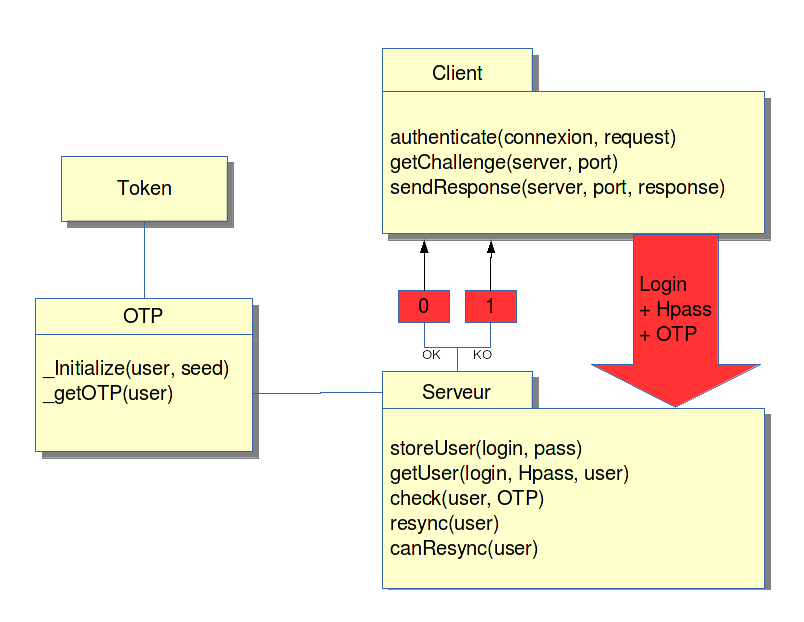
\includegraphics[scale=0.1]{img/architecture.png} % À MODIFIER !
 \caption{Schéma de l'architecture logicielle}
\end{figure}

\end{frame}


%------------------------------------------------
\section{Test et vérification}
%------------------------------------------------

\subsection{Vérification}

\begin{frame}
  \frametitle{Vérification}
  Chaque partie de developpement fera le cadre d'un verification 
\end{frame}

\subsection{Tests}

\begin{frame}
  \frametitle{Tests}
  Nous ferons des test de qualité afin de ...
\end{frame}


%------------------------------------------------
\section{Plan de développement}
%------------------------------------------------
\begin{frame}
  \begin{block}{Planning Poker}
    \begin{figure}
      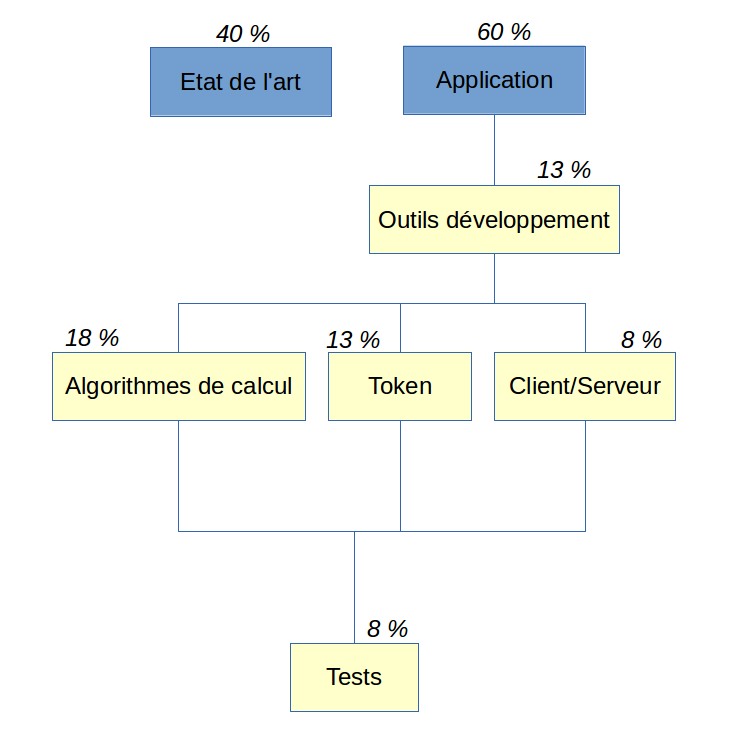
\includegraphics[scale=0.1]{img/planningpoker.png} % À MODIFIER !
      \caption{Planning poker}
    \end{figure}
  \end{block}
\end{frame}

\begin{frame}
  \begin{block}{Diagramme de gantt}
    \begin{figure}
      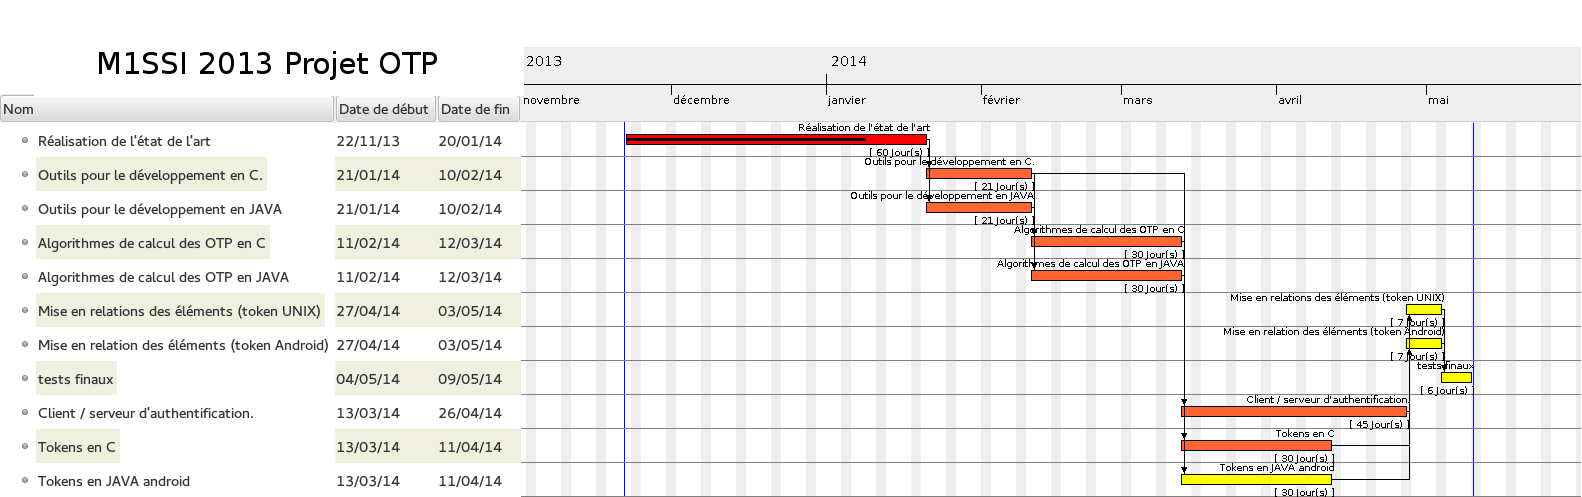
\includegraphics[scale=0.1]{img/gantt.png} % À MODIFIER !
      \caption{Planning des étapes du projet}
    \end{figure}
  \end{block}
\end{frame}

%------------------------------------------------
\section{Gestion des risques}
%------------------------------------------------
% Synthèse des risques ? On ne recopies pas tout les risque je suppose


%------------------------------------------------
\section{Conclusion}
%------------------------------------------------

\subsection{En Conclusion}

\begin{frame}
\frametitle{Conclusion}
  Le projet est réalisable...ou pas.
\end{frame}



%------------------------------------------------
\end{document}